\chapter{Conclusions}
\label{chap:conclusions}
\minitoc \mtcskip \noindent

\section{Difficulties}
%IMPORTANT
%Maybe move to the approach
Mention the initial thing we wanted to do: to use some metrics to compare our implementation with others from the state of the art.
Mention why we could not do it: NO ONE ANSWERED WITH THE METRICS :( Contacts did not go through as expected!

\section{}

% Nao ha grande baseline para comparar; há que restringir o ambito e o estudo foi feito para ser baseado nestas consideraçoes; 

%These conclusions are for PDIS; so they will close this delivery and may anticipate the expected results of the dissertation. Include the tasks and a Gantt diagram with the plan.
The dissertation focuses on finding out how applicable Blockchain is to the supply chain industry and to SCM, and there are many variables to consider. Many companies have already started working on projects similar to what is trying to be accomplished here, though with a higher focus on financial benefits than on the research itself (many of the examples given were of companies using Ethereum and its tokens). These solutions have not yet been proved and are also taking their initial steps. The main focus of this dissertation is to develop a proof-of-concept that indeed Blockchain can improve SCM in some form, and also give an insight on how this might be achieved. 

\section{Future Work}

Future work: The work here done was much more introductory in nature, and explored the requirements and their satisfaction as a whole. Additionaly, the maturity of the tools used was questionable. 
Future work might include:
\begin{itemize}
	\item Taking specific requirements from the most important requirements on the list and research on using blockchain to successfully apply them as enhancements:
	\begin{itemize}
		\item Financial applications, payments and contractual agreements;
		\item "Applying Blockchain as a financial alternative in the Supply Chain" could even be a new thesis derived out of this one;
	\end{itemize}
	\item Research and attempt to use different frameworks to fulfill the same requirements that were elicited in this dissertation;
    \item Research on different architectures
\end{itemize} 

%Nao usar situaçoes hipoteticas
%USAR OUTRAS FERRAMENTAS
%COMPARAR COM CLOUD E OUTRAS ARQUITETURAS
%VALIDAR PROTOTIPO COM PESSOAS REAIS

The research for this dissertation is divided into six steps, described in Table \ref{table:gantt_chart} and illustrated by Figure \ref{fig:gantt_chart}. The research started with the literature review, which presents some important insights, frameworks as well as some important design aspects and decisions to take while developing a model for a Blockchain-driven supply chain project.

These aspects will be taken into account for the next steps. First, adapting and creating a Blockchain integration model, by making some decisions on the design and frameworks to be used. Then, a small integration project will be built based on this model.

In the final part of the project, its applicability and performance will be evaluated. The developed system itself is a proof-of-concept, which, already proves that such a concept might work, but it is important to measure how it fares against the traditional systems used in supply chain. This evaluation is done in two different parts: the first consists on evaluating functionality, and checking which functionalities are added or subtracted by using blockchain; the second part consists in using performance metrics to evaluate this dissertation's solution against the baseline of a traditional solution, like a centralized system. The metrics used to evaluate this include, but are not limited to:
\begin{itemize}
\item Throughput - processed transactions per second
\item Latency - average time to process a single transaction
\item Latency volatility - measure of the variety of latency
\item Security - qualitative evaluation that includes items such as immutability, denial of service resilience, trust and fraud protection, confidentiality and access control
\item Hardware requirements - how much hardware is needed, and how powerful
\item Scalability - number of nodes, transactions, users and how much the system can stretch these numbers
\end{itemize}

%\todo{fcorreia: do you have already any additional ideas about the baseline that you will be comparing to? it'd be great if you could provide a bit more detail about this; will it be a non-blockchain-based distributed system? (e.g., a microservice-based system, or a system based on a replicated datastore) Will it be simply a "normal" centralized system? Depending on the baseline that you choose the conclusions that you will be able to reach will be quite different}

Finally, the model might have to be recalibrated, taking into account the results gathered from these metrics. The values of the model might have to be changed iteratively, until a satisfying solution is achieved, if possible.

%%%%%%%%%%%%%%%%%%%%%%%% TABLE %%%%%%%%%%%%%%%%%%%%%%%%%%%%%%%%%

% Please add the following required packages to your document preamble:
% \usepackage[table,xcdraw]{xcolor}
% If you use beamer only pass "xcolor=table" option, i.e. \documentclass[xcolor=table]{beamer}
\begin{table}[]
\centering
\begin{tabular}{l|r|r|}
\cline{2-3}
                                                                                                  & \multicolumn{1}{l|}{{\color[HTML]{343434} \textbf{Starting}}} & \multicolumn{1}{l|}{{\color[HTML]{343434} \textbf{Ending}}} \\ \hline
\multicolumn{1}{|l|}{{\color[HTML]{343434} 1. Literature Review}}                                 & 1 Jan 2018                                                    & 9 Feb 2018                                                  \\ \hline
\multicolumn{1}{|l|}{{\color[HTML]{343434} 2. Decide on the features and design the model}}       & 10 Feb 2018                                                   & 5 Mar 2018                                                  \\ \hline
\multicolumn{1}{|l|}{{\color[HTML]{343434} 3. Create a small integration project}}                & 6 Mar 2018                                                    & 15 Apr 2018                                                 \\ \hline
\multicolumn{1}{|l|}{{\color[HTML]{343434} 4. Evaluate its applicability and performance}}        & 16 Apr 2018                                                   & 29 Apr 2018                                                 \\ \hline
\multicolumn{1}{|l|}{{\color[HTML]{343434} 5. Recalibrate the model's values, given the results}} & 30 Apr 2018                                                   & 14 May 2018                                                 \\ \hline
\multicolumn{1}{|l|}{{\color[HTML]{343434} 6. Finalize the dissertation document}}                & 15 May 2018                                                   & 22 Jun 2018                                                 \\ \hline
\end{tabular}
\caption{Work plan description for figure \ref{fig:gantt_chart}}
\label{table:gantt_chart}
\end{table}



%%%%%%%%%%%%%%%%%%%%%%%%%%%%%%%%%%%%%%%%%%%%%%%%%%%%%%%%%%%%%%%%
\begin{figure}[ht]
\centering
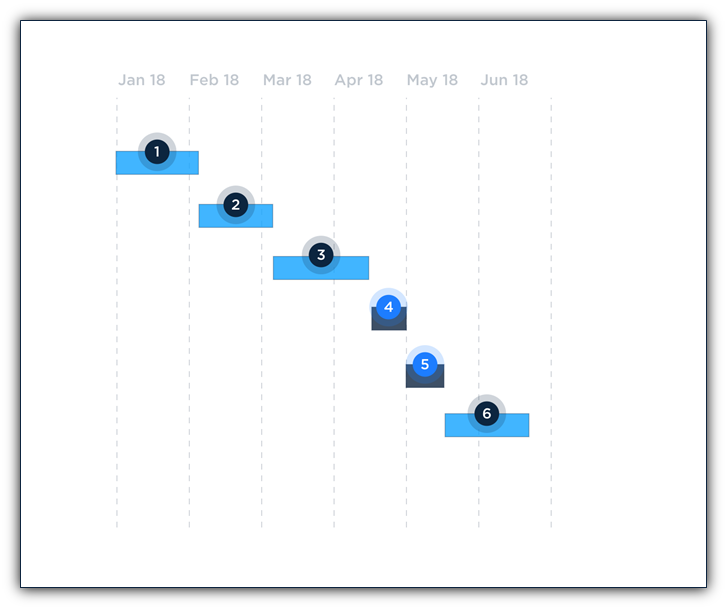
\includegraphics[scale=0.75]{media/gantt.png}
\caption{Research work plan}
\label{fig:gantt_chart}
\end{figure}

\section{Expected Results}
From this dissertation, it is expected that a proof-of-concept system with certain characteristics will emerge. The results will be analyzed to check if the system follows the parameters we are looking for.

For instance, it should be able to integrate information from various sources into a single place. This information should be available at any time, anywhere. It should be cryptographically secure, immutable, and easy and quick to share.

In the end, we need to analyze the results with the given metrics and ascertain whether there is a significant increase in performance and functionality that would justify using blockchain in a real supply chain.

%\todo{fcorreia: I'd expect to see here a list of contributions of your thesis. You do mention them, but a) I think they would be clearer to read as a list, b) you may be currently missing a few. I see at least 3 or 4, for example: a study of important design considerations for SCMSs, a study of important design considerations for blockchains, a prototype, an analysis of the benefits and liabilities of supporting a SCMS with a blockchain}

% pedro: I don't think a list is a good representation for the conclusion, especially when it is the ending of the document. And I don't know what other results to expect, I've written the ones we had discussed previously.


